\documentclass{beamer}
\usepackage[utf8]{inputenc} 
\usepackage[T1]{fontenc}    
\usepackage[brazil,english]{babel} 
\usepackage{apacite}
\usepackage{ragged2e}
\usepackage{color}
\usepackage{mathrsfs}
\usepackage{amsfonts}
\usepackage{amssymb}
\usepackage{amsmath}
\usetheme{Frankfurt}

%\usetheme{Darmstadt}
\usecolortheme{dove}
%\usecolortheme{beetle}
\usefonttheme{professionalfonts}
%\usefonttheme{structureitalicserif}
%\setbeamertemplate{footline}[frame number]
%\usefonttheme[onlymath]{serif} % fonte modo matematico
% Titulo

\usepackage{graphicx}
\usepackage{caption}
\usepackage{subcaption}

\setbeamertemplate{navigation symbols}{}

\title[\sc{Trabalho de Conclusão de Curso}]{{\normalsize Trabalho de Conclusão de Curso} \\ \vspace*{2mm} {\bf Simulação de Algoritmos Distribuídos Aplicados ao Cálculo do PageRank}}
\author[Oscar Neiva E. Neto]{Oscar Neiva E. Neto \\ \vspace{2mm} {\footnotesize Orientador: D.Sc. Eduardo Krempser\\ Coorientador: D.Sc. Marcos Garcia Todorov}}
\institute[FAETERJ]{Faculdade de Educação Tecnológica do Estado do Rio de Janeiro - FAETERJ Petrópolis\\ 
Laboratório Nacional de Computação Científica - LNCC}  % opcional
\logo{
\includegraphics[height=0.8cm]{figures/faeterjbw.png}}
\date{}

\defbeamertemplate*{footline}{shadow theme}{%
\leavevmode%
\hbox{\begin{beamercolorbox}[wd=.5\paperwidth,ht=2.5ex,dp=1.125ex,leftskip=.3cm plus1fil,rightskip=.3cm]{author in head/foot}%
    \usebeamerfont{author in head/foot}\hfill\insertshortauthor
\end{beamercolorbox}%
\begin{beamercolorbox}[wd=.4\paperwidth,ht=2.5ex,dp=1.125ex,leftskip=.3cm,rightskip=.3cm plus1fil]{title in head/foot}%
    \usebeamerfont{title in head/foot}\insertshorttitle\hfill%
\end{beamercolorbox}%
\begin{beamercolorbox}[wd=.1\paperwidth,ht=2.5ex,dp=1.125ex,leftskip=.3cm,rightskip=.3cm plus1fil]{mycolor}%
\hfill\insertframenumber\,/\,\inserttotalframenumber
\end{beamercolorbox}}%
\vskip0pt%
}

\justifying

\begin{document}
%%%%%%%%%%%%%%%%%%%%%%%%%%%%%%%%%%%%%%%%%%%%%%%%%%%%%%%%%%%%%%%%%%%%%%%%%%%%%%%%%%%%%%%%%%%%%%%%%%%%%%%%%%%%
%%%%%%%%%%%%%%%%%%%%%%%%%%%%%%%%%%%%%%%%%%%%%%%%%%%%%%%%%%%%%%%%%%%%%%%%%%%%%%%%%%%%%%%%%%%%%%%%%%%%%%%%%%%%
\begin{frame}
  	\titlepage
\end{frame}
%%%%%%%%%%%%%%%%%%%%%%%%%%%%%%%%%%%%%%%%%%%%%%%%%%%%%%%%%%%%%%%%%%%%%%%%%%%%%%%%%%%%%%%%%%%%%%%%%%%%%%%%%%%%
%%%%%%%%%%%%%%%%%%%%%%%%%%%%%%%%%%%%%%%%%%%%%%%%%%%%%%%%%%%%%%%%%%%%%%%%%%%%%%%%%%%%%%%%%%%%%%%%%%%%%%%%%%%%
\begin{frame}
	\frametitle{Índice}
	\tableofcontents
\end{frame}
%%%%%%%%%%%%%%%%%%%%%%%%%%%%%%%%%%%%%%%%%%%%%%%%%%%%%%%%%%%%%%%%%%%%%%%%%%%%%%%%%%%%%%%%%%%%%%%%%%%%%%%%%%%%
%%%%%%%%%%%%%%%%%%%%%%%%%%%%%%%%%%%%%%%%%%%%%%%%%%%%%%%%%%%%%%%%%%%%%%%%%%%%%%%%%%%%%%%%%%%%%%%%%%%%%%%%%%%%
\begin{frame}
	\section{Introdução}
	\subsection{}
	\frametitle{Motivação e Objetivo}

\begin{itemize}
	\item A motivação para os estudos no tema parte dos problemas relacionados a simulação do algoritmo \textit{PageRank}.
	\vspace{0.5cm}	
	\item O trabalho consiste no estudo e simulação de sistemas sujeitos a saltos markovianos.
\end{itemize}		 

\end{frame}
%%%%%%%%%%%%%%%%%%%%%%%%%%%%%%%%%%%%%%%%%%%%%%%%%%%%%%%%%%%%%%%%%%%%%%%%%%%%%%%%%%%%%%%%%%%%%%%%%%%%%%%%%%%%
%%%%%%%%%%%%%%%%%%%%%%%%%%%%%%%%%%%%%%%%%%%%%%%%%%%%%%%%%%%%%%%%%%%%%%%%%%%%%%%%%%%%%%%%%%%%%%%%%%%%%%%%%%%%
\begin{frame}
	\section{O Algoritmo PageRank}
	\subsection{}
	\frametitle{O Algoritmo PageRank}

\begin{itemize}
	\item A proposta do \textit{PageRank}\footnote{\tiny \justifying Brin, Sergey and Page, Lawrence, The anatomy of a large-scale hypertextual web search engine, 1998.}.
	\vspace{0.2cm}	
	\item O grau de importância das páginas.
	\vspace{0.2cm}
	\item O Sistema de Busca e o \textit{PageRank}.
\end{itemize}	

\vspace{0.3cm}
	
\begin{figure}[!htb]
	\centering
	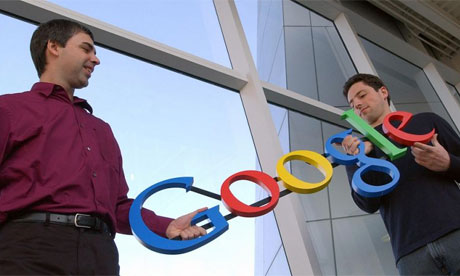
\includegraphics[scale=0.23]{figures/larry}
	\hspace{0.1cm}
	
\includegraphics[scale=0.2]{figures/google}\\
	%\caption{Sergey Brin e Lawrence Page.}
	{\scriptsize Criadores do \textit{PageRank} e barra de pesquisa do Google}
	%\label{larry}
\end{figure}	 

\end{frame}
%%%%%%%%%%%%%%%%%%%%%%%%%%%%%%%%%%%%%%%%%%%%%%%%%%%%%%%%%%%%%%%%%%%%%%%%%%%%%%%%%%%%%%%%%%%%%%%%%%%%%%%%%%%%
%%%%%%%%%%%%%%%%%%%%%%%%%%%%%%%%%%%%%%%%%%%%%%%%%%%%%%%%%%%%%%%%%%%%%%%%%%%%%%%%%%%%%%%%%%%%%%%%%%%%%%%%%%%%
\begin{frame}
	%\section{O Algoritmo PageRank}
	%\subsection{As Ferramentas de Busca}
	\frametitle{As Ferramentas de Busca}
	
\begin{itemize}
	\item Da \textit{World Wide Web Worm} em 1994 até 2016.
	\vspace{0.3cm}
	\item Nos útimos 20 anos a \textit{Web} vem ganhando 240.000.000 páginas por ano. 
\end{itemize}	
	
\
\begin{table}[!htb]
\centering
\begin{tabular}{lllll}
Ano & Buscador & Nº de Páginas Indexadas\\
1994 & WWWW & 110 mil\\
1997 & AltaVista & 100 milhões\\
1998 & Google & 518 milhões\\
2016 & Google & 4.8 bilhões
\end{tabular}
\end{table}
	
\end{frame}
%%%%%%%%%%%%%%%%%%%%%%%%%%%%%%%%%%%%%%%%%%%%%%%%%%%%%%%%%%%%%%%%%%%%%%%%%%%%%%%%%%%%%%%%%%%%%%%%%%%%%%%%%%%%
%%%%%%%%%%%%%%%%%%%%%%%%%%%%%%%%%%%%%%%%%%%%%%%%%%%%%%%%%%%%%%%%%%%%%%%%%%%%%%%%%%%%%%%%%%%%%%%%%%%%%%%%%%%%
\begin{frame}
	%\section{O Algoritmo PageRank}
	%\subsection{Os Desafios do PageRank}
	\frametitle{Os Desafios do PageRank}
	
\begin{itemize}
	\item A massividade da \textit{Web} e a dificuldade do cálculo.
	\vspace{0.2cm}		
	\item A navegação entre páginas desconexas.
	\vspace{0.2cm}	
	\item A página Buraco Negro.
\end{itemize}	

\begin{figure}[!htb]
	\centering
	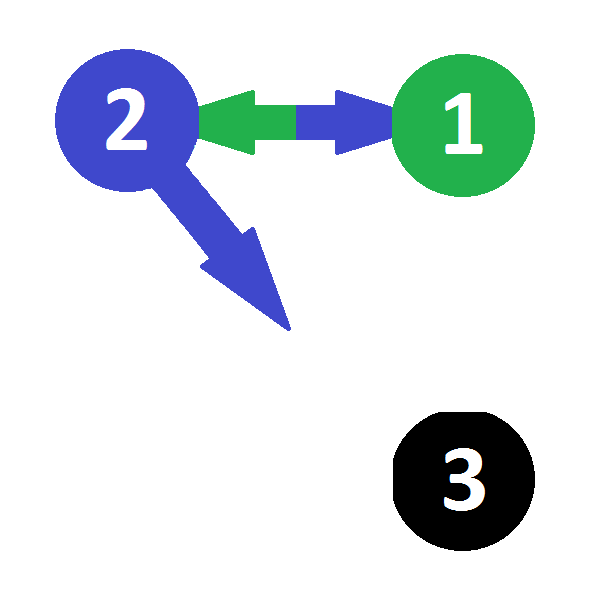
\includegraphics[scale=0.20]{figures/blackhole1}
	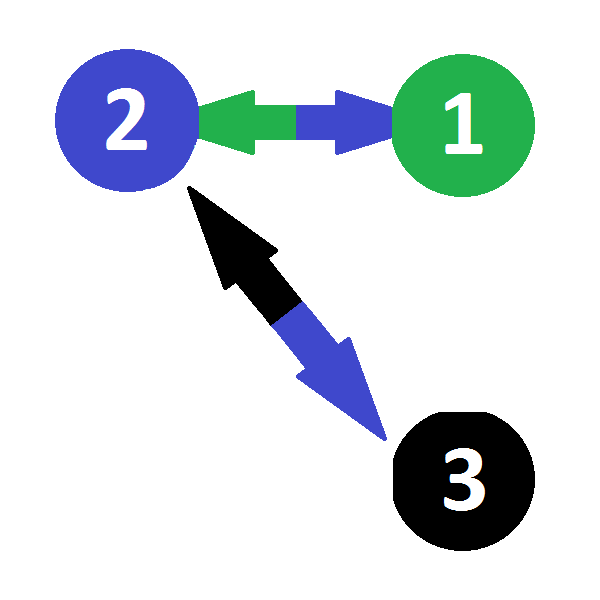
\includegraphics[scale=0.20]{figures/blackhole2}\\
	%\caption{Sergey Brin e Lawrence Page.}
	{\scriptsize O Buraco Negro da \textit{Web}}
	%\label{larry}
\end{figure}	 

\end{frame}
%%%%%%%%%%%%%%%%%%%%%%%%%%%%%%%%%%%%%%%%%%%%%%%%%%%%%%%%%%%%%%%%%%%%%%%%%%%%%%%%%%%%%%%%%%%%%%%%%%%%%%%%%%%%
%%%%%%%%%%%%%%%%%%%%%%%%%%%%%%%%%%%%%%%%%%%%%%%%%%%%%%%%%%%%%%%%%%%%%%%%%%%%%%%%%%%%%%%%%%%%%%%%%%%%%%%%%%%%
\begin{frame}
	\section{Definição dos Modelos}
	\subsection{A Matriz Hiperlink}
	\frametitle{A Matriz Hiperlink}

\vspace{-1cm}

\begin{figure}[!htb]
	\centering
	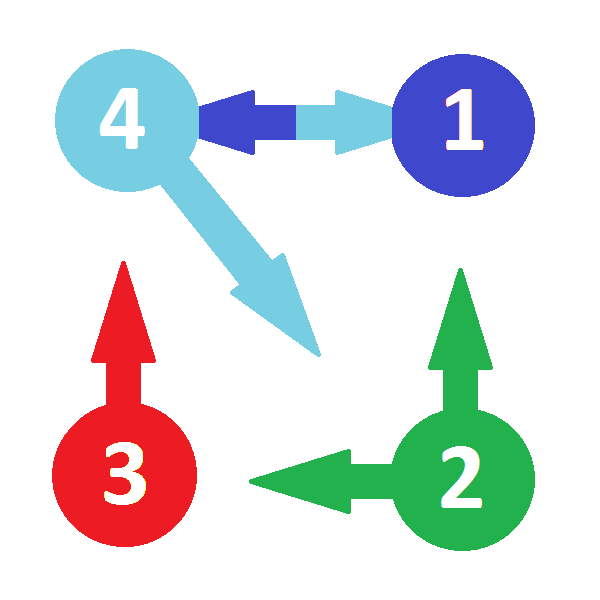
\includegraphics[scale=0.2]{figures/grafo}\\
	%\caption{Sergey Brin e Lawrence Page.}
	{\scriptsize Grafo representando \textit{links} entre p\'aginas da \textit{web}}
	%\label{larry}
\end{figure}	

\begin{equation}
A = \begin{pmatrix}
 0 & 1/2 & 0 & 1/2 \\
 0 &  0  & 0 & 1/2 \\
 0 & 1/2 & 0 &  0  \\
 1 &  0  & 1 &  0
\end{pmatrix}
\end{equation}		
\end{frame}
%%%%%%%%%%%%%%%%%%%%%%%%%%%%%%%%%%%%%%%%%%%%%%%%%%%%%%%%%%%%%%%%%%%%%%%%%%%%%%%%%%%%%%%%%%%%%%%%%%%%%%%%%%%%
%%%%%%%%%%%%%%%%%%%%%%%%%%%%%%%%%%%%%%%%%%%%%%%%%%%%%%%%%%%%%%%%%%%%%%%%%%%%%%%%%%%%%%%%%%%%%%%%%%%%%%%%%%%%
\begin{frame}
	%\section{Definição dos Modelos}
	%\subsection{A Matriz Hiperlink}
	\frametitle{A Matriz Hiperlink}
	
\begin{itemize}
\item $n$: n\'os, que representam as p\'aginas. A navega\c{c}\~ao \'e ent\~ao representada atrav\'es de uma cadeia de Markov com espa\c{c}o de estados discreto de dimens\~ao $n$.

\vspace{0.3cm}	
	
\item $\mathcal{E}$: arestas, que representam os \textit{links}. Para o caso de um v\'ertice $i$ estar conectado a um $j$, tem-se que $(i,j) \in \mathcal{E}$.
\end{itemize}
	
\begin{equation}
a_{ij} = \begin{cases}
\dfrac{1}{n_i}, & \text{caso}\, (i,j)\in \mathcal{E},\\
0, & \text{caso contr\'ario}.
\end{cases}
\end{equation}	
	
\end{frame}
%%%%%%%%%%%%%%%%%%%%%%%%%%%%%%%%%%%%%%%%%%%%%%%%%%%%%%%%%%%%%%%%%%%%%%%%%%%%%%%%%%%%%%%%%%%%%%%%%%%%%%%%%%%%
%%%%%%%%%%%%%%%%%%%%%%%%%%%%%%%%%%%%%%%%%%%%%%%%%%%%%%%%%%%%%%%%%%%%%%%%%%%%%%%%%%%%%%%%%%%%%%%%%%%%%%%%%%%%
\begin{frame}
	%\section{Definição dos Modelos}
	\subsection{O Power Method}
	\frametitle{O Power Method}
	
\begin{itemize}

\item Um m\'etodo para obten\c{c}\~ao do \textit{PageRank} \'e o chamado \textit{Power Method}\footnote{\tiny \justifying Ishii, Hideaki and Tempo, Roberto, The pagerank problem, multiagent consensus, and web aggregation: A systems and control viewpoint, 2014.}.
		
\vspace{0.5cm}

\item O \textit{PageRank} é o ponto fixo da seguinte recursão:
%
\begin{equation}
	x(k+1) = Ax(k),\: k\geq0,\: \text{com} \: x(0) = x_0,
\end{equation}
%
onde $x_0 \in \mathbb{R}^{n \times 1}$ \'e uma condi\c{c}\~ao inicial positiva de soma igual a um.

\end{itemize}
	
\end{frame}
%%%%%%%%%%%%%%%%%%%%%%%%%%%%%%%%%%%%%%%%%%%%%%%%%%%%%%%%%%%%%%%%%%%%%%%%%%%%%%%%%%%%%%%%%%%%%%%%%%%%%%%%%%%%
%%%%%%%%%%%%%%%%%%%%%%%%%%%%%%%%%%%%%%%%%%%%%%%%%%%%%%%%%%%%%%%%%%%%%%%%%%%%%%%%%%%%%%%%%%%%%%%%%%%%%%%%%%%%
\begin{frame}
	%\section{Definição dos Modelos}
	%\subsection{Questões de Convergência do Power Method}
	\frametitle{Questões de Convergência do Power Method}

\begin{itemize}
\item Caso a matriz $A$ seja irredutível, independente da condição inicial é atingida a distribuição limite.
\vspace{0.2cm}
\item Diz-se que $A$ é irredutivel se sempre existe um caminho ligando dois nós quaisquer.
\end{itemize}

\vspace{0.1cm}

\begin{center}
$A = \begin{pmatrix}
 0 & 1/2 & 0 & 1/2 \\
 0 &  0  & 0 & 1/2 \\
 0 & 1/2 & 0 &  0  \\
 1 &  0  & 1 &  0
\end{pmatrix}$
\hspace{1cm}
$x^* = \begin{pmatrix}
 0.3\\
 0.2\\
 0.1\\
 0.4
\end{pmatrix}$
\end{center}

\begin{figure}[!htb]
	\centering
	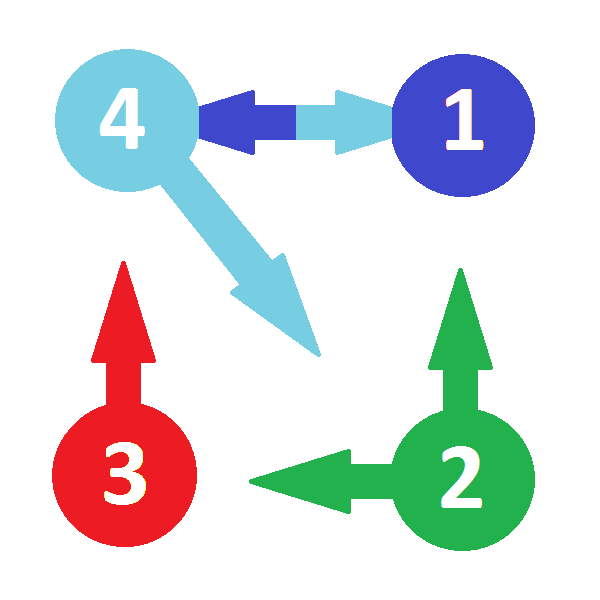
\includegraphics[scale=0.16]{figures/grafo}\\
	%\caption{Sergey Brin e Lawrence Page.}
	%{\scriptsize Grafo representando \textit{links} entre p\'aginas da \textit{web}}
	%\label{larry}
\end{figure}	
	
\end{frame}
%%%%%%%%%%%%%%%%%%%%%%%%%%%%%%%%%%%%%%%%%%%%%%%%%%%%%%%%%%%%%%%%%%%%%%%%%%%%%%%%%%%%%%%%%%%%%%%%%%%%%%%%%%%%
%%%%%%%%%%%%%%%%%%%%%%%%%%%%%%%%%%%%%%%%%%%%%%%%%%%%%%%%%%%%%%%%%%%%%%%%%%%%%%%%%%%%%%%%%%%%%%%%%%%%%%%%%%%%
\begin{frame}
	%\section{Definição dos Modelos}
	\subsection{Teleportation Model}
	\frametitle{Teleportation Model}

\begin{itemize}
	\item Embora a simplicidade do \textit{Power Method} o torne atraente, ele pode apresentar problemas de convergência.
	\vspace{0.2cm}	
	\item O Teleportation promove exploração, sem afetar o \textit{PageRank}.
\end{itemize}		
	
\begin{figure}[!htb]
	\centering
	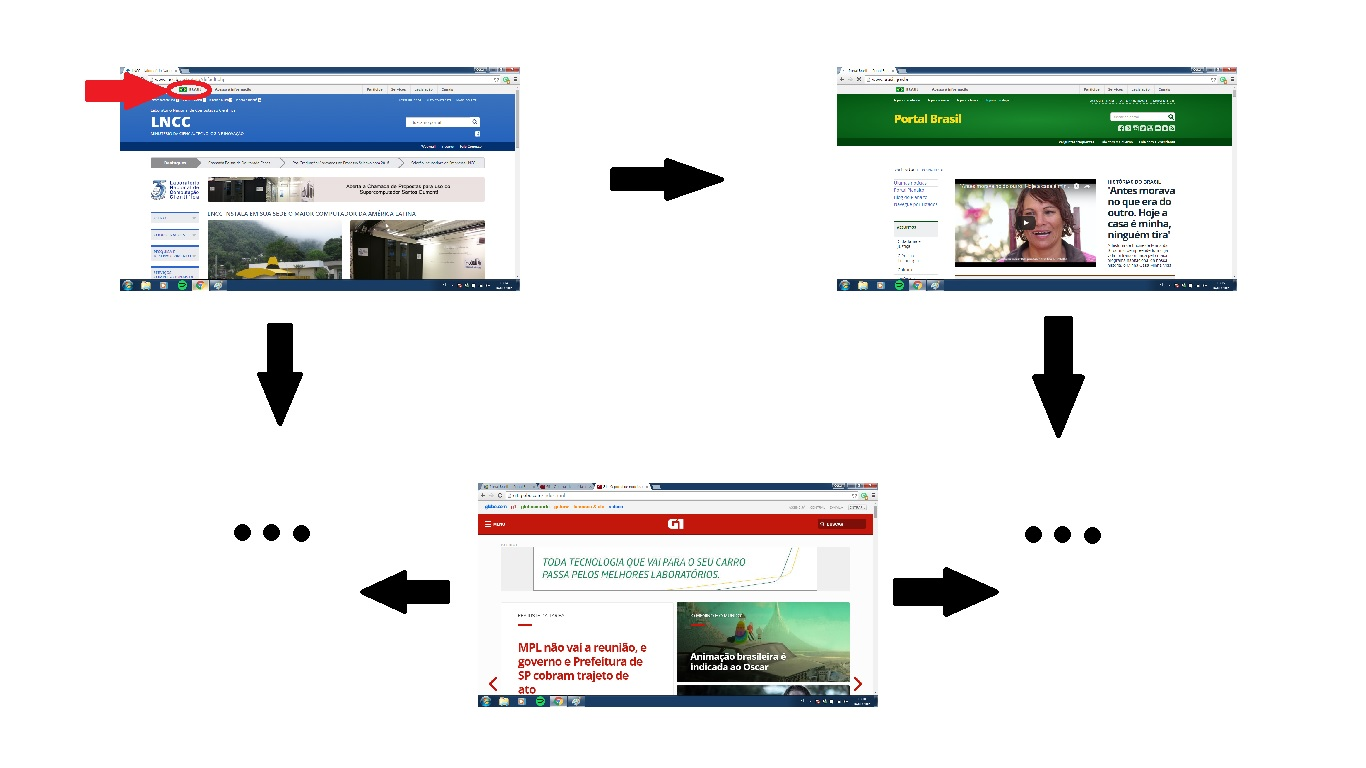
\includegraphics[scale=0.26]{figures/tele}\\
	%\caption{Sergey Brin e Lawrence Page.}
	%{\scriptsize Grafo representando \textit{links} entre p\'aginas da \textit{web}}
	%\label{larry}
\end{figure}		
	
\end{frame}
%%%%%%%%%%%%%%%%%%%%%%%%%%%%%%%%%%%%%%%%%%%%%%%%%%%%%%%%%%%%%%%%%%%%%%%%%%%%%%%%%%%%%%%%%%%%%%%%%%%%%%%%%%%%
%%%%%%%%%%%%%%%%%%%%%%%%%%%%%%%%%%%%%%%%%%%%%%%%%%%%%%%%%%%%%%%%%%%%%%%%%%%%%%%%%%%%%%%%%%%%%%%%%%%%%%%%%%%%
\begin{frame}
	%\section{Definição dos Modelos}
	%\subsection{\textit{Teleportation Model}}
	\frametitle{\textit{Teleportation Model}}

\begin{itemize}	
	\item O \textit{Teleportation Model} \'e uma estrat\'egia reconhecida para que, atrav\'es de uma pequena modifica\c{c}\~ao na matriz $A$, o m\'etodo convirja globalmente.
	
\begin{equation}
	M = (1-m)A + \frac{m}{n} \textbf{11}^T
\end{equation}
 
	\begin{itemize}
	\item $m \in (0,1)$
	\item $M \in \mathbb{R}^{n \times n}$
	\item $\textbf{1} \in \mathbb{R}^{n \times 1}$
	\end{itemize}
\end{itemize}		
	
\end{frame}
%%%%%%%%%%%%%%%%%%%%%%%%%%%%%%%%%%%%%%%%%%%%%%%%%%%%%%%%%%%%%%%%%%%%%%%%%%%%%%%%%%%%%%%%%%%%%%%%%%%%%%%%%%%%
%%%%%%%%%%%%%%%%%%%%%%%%%%%%%%%%%%%%%%%%%%%%%%%%%%%%%%%%%%%%%%%%%%%%%%%%%%%%%%%%%%%%%%%%%%%%%%%%%%%%%%%%%%%%
\begin{frame}
	%\section{Definição dos Modelos}
	\subsection{O Modelo dos Algoritmos Distribuídos}
	\frametitle{O Modelo dos Algoritmos Distribuídos}
	
\begin{itemize}
\item Tornar o c\'alculo menos custoso e factível.
\vspace{0.2cm}
\item Explorar os recursos computacionais dos servidores.
\vspace{0.2cm}
\item Emprego de algoritmos distribu\'idos\footnote{\tiny \justifying Lei, Jianjun and Chen, Han-Fu, Distributed Randomized PageRank Algorithm Based on Stochastic Approximation, 2015.}.
\end{itemize}
\vspace{0.4cm}
\begin{figure}[!htb]
	\centering
	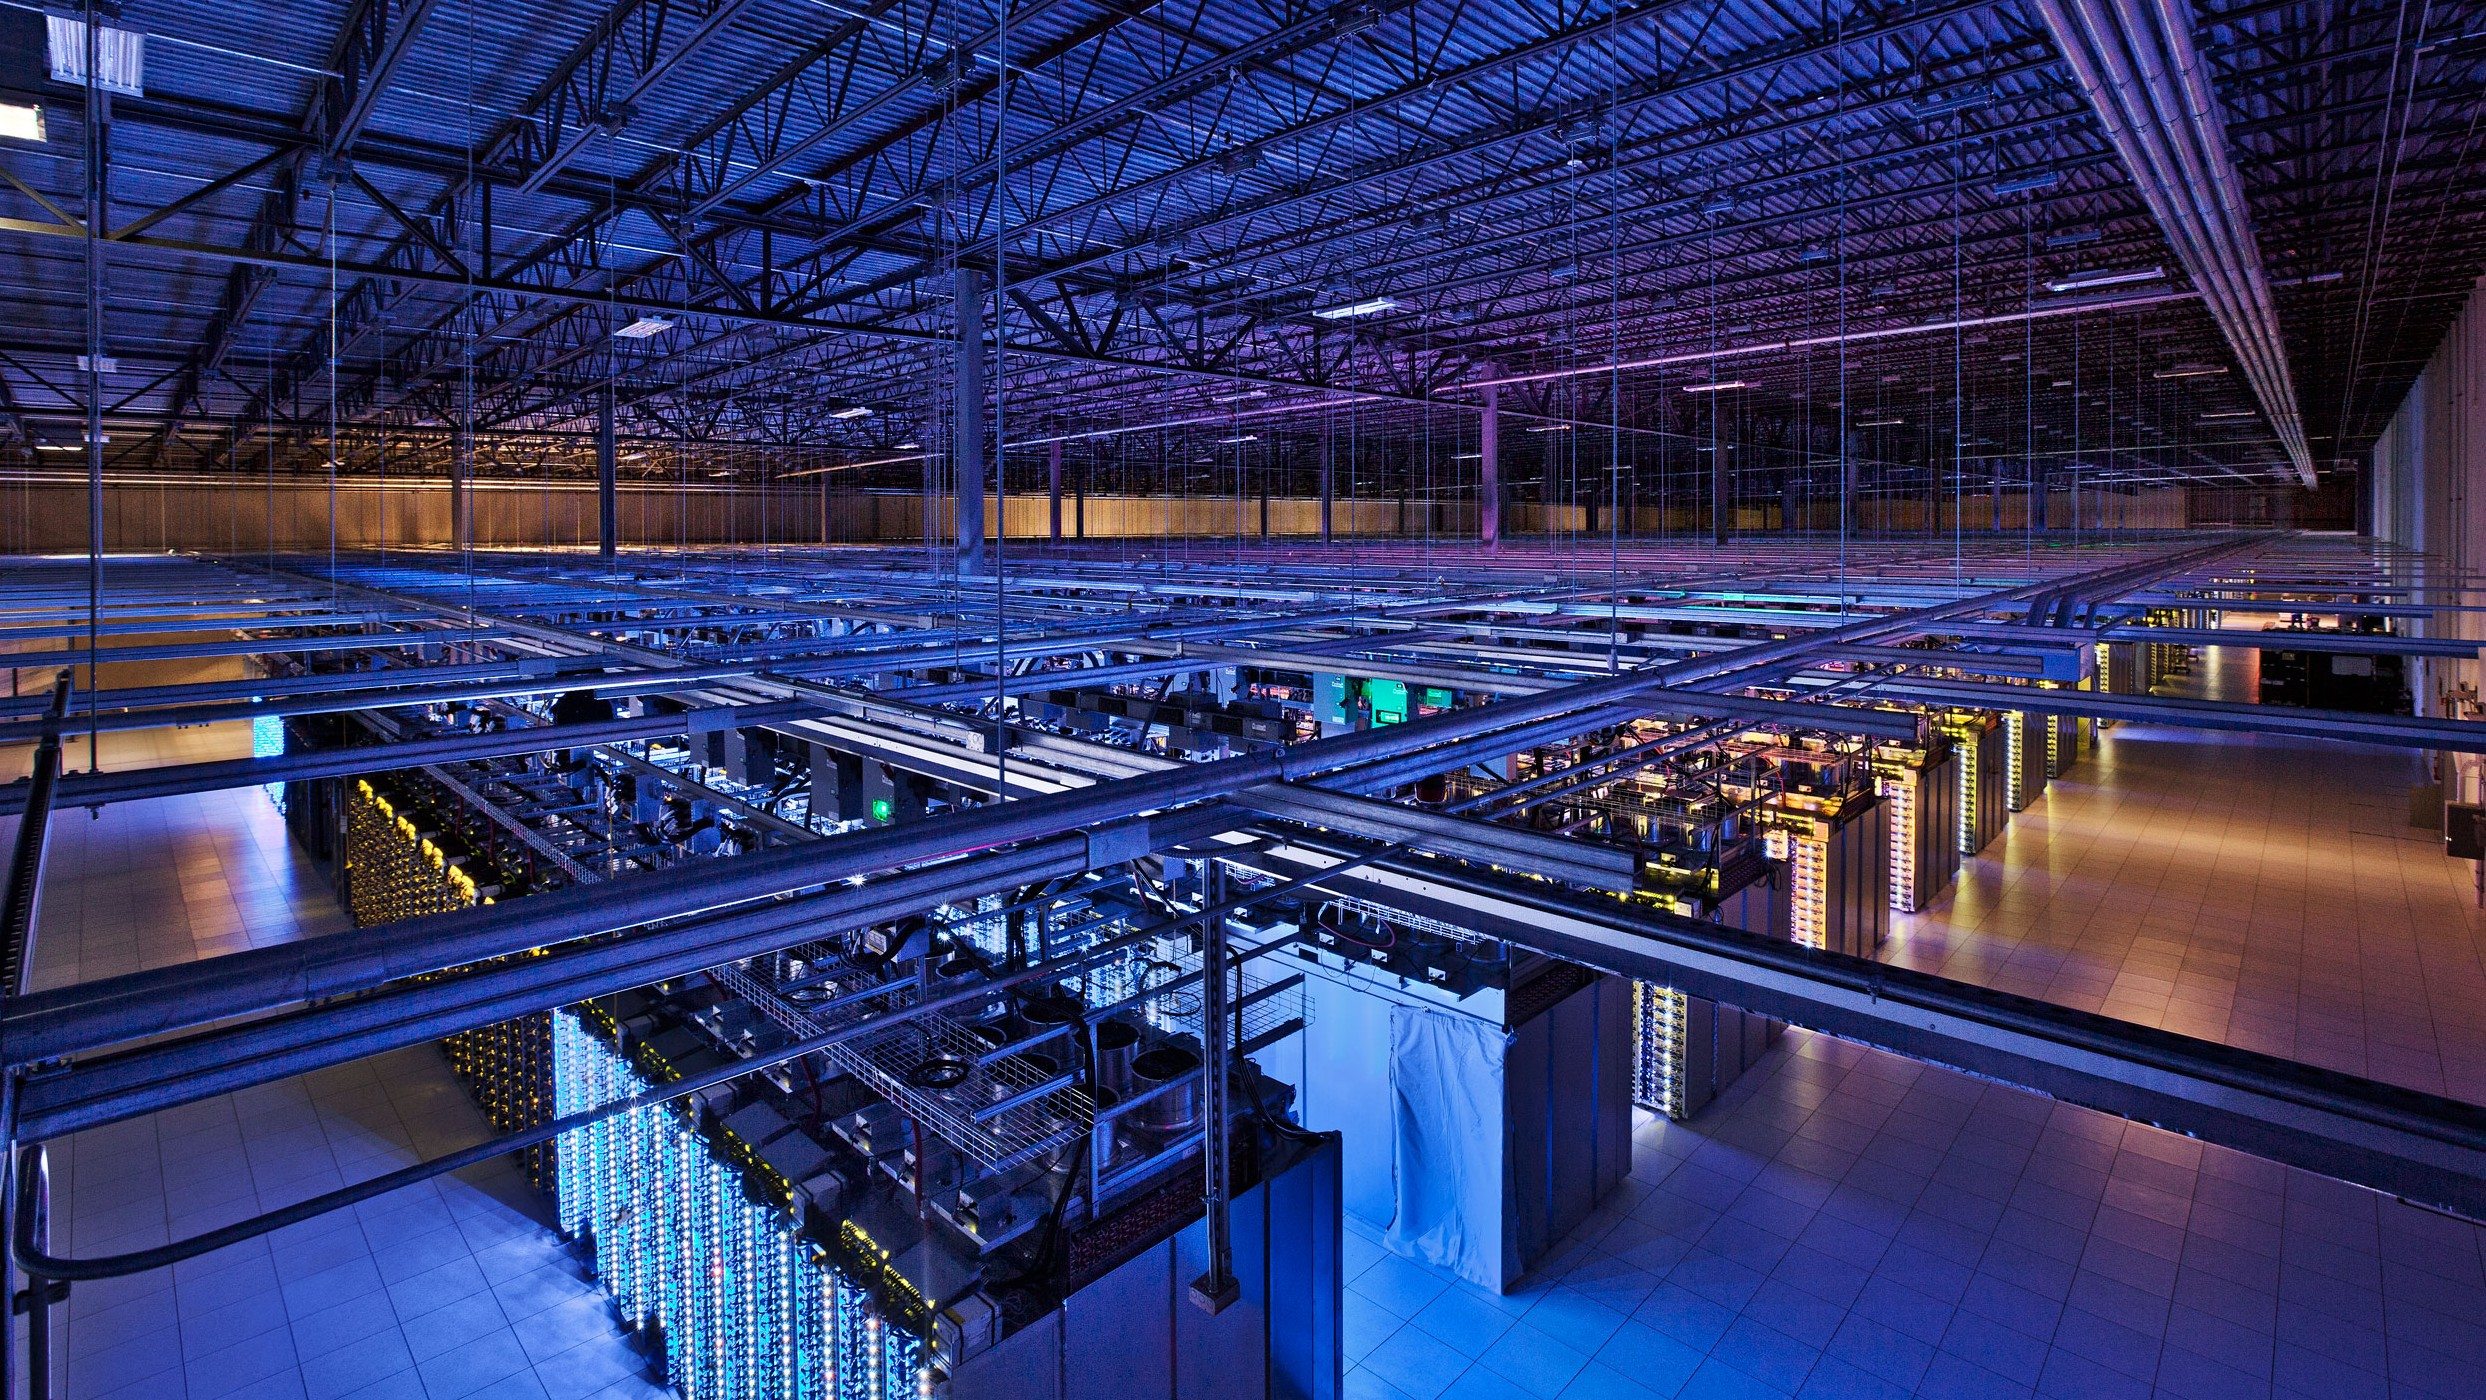
\includegraphics[scale=0.07]{figures/cluster}\\
	%\caption{Sergey Brin e Lawrence Page.}
	{\scriptsize Cluster da Google.}
	%\label{larry}
\end{figure}	

\end{frame}
%%%%%%%%%%%%%%%%%%%%%%%%%%%%%%%%%%%%%%%%%%%%%%%%%%%%%%%%%%%%%%%%%%%%%%%%%%%%%%%%%%%%%%%%%%%%%%%%%%%%%%%%%%%%
%%%%%%%%%%%%%%%%%%%%%%%%%%%%%%%%%%%%%%%%%%%%%%%%%%%%%%%%%%%%%%%%%%%%%%%%%%%%%%%%%%%%%%%%%%%%%%%%%%%%%%%%%%%%
\begin{frame}
	%\section{Definição dos Modelos}
	%\subsection{O Modelo dos Algoritmos Distribuídos}
	\frametitle{O Modelo dos Algoritmos Distribuídos}

\begin{equation}\nonumber
A = \begin{pmatrix}
 0 & 1/2 & 0 & 1/2 \\
 0 &  0  & 0 & 1/2 \\
 0 & 1/2 & 0 &  0  \\
 1 &  0  & 1 &  0
\end{pmatrix}
\end{equation}
\vspace{0.4cm}
\begin{equation}\nonumber
A_1 = \begin{pmatrix}
 0 &  0  & 0 &  0 \\
 0 &  1  & 0 &  0 \\
 0 &  0  & 1 &  0  \\
 1 &  0  & 0 &  1
\end{pmatrix}
%
A_2 = \begin{pmatrix}
 1 & 1/2 & 0 &  0 \\
 0 &  0  & 0 &  0 \\
 0 & 1/2 & 1 &  0  \\
 0 &  0  & 0 &  1
\end{pmatrix}
\end{equation}

\begin{equation}\nonumber
A_3 = \begin{pmatrix}
 1 &  0  & 0 &  0 \\
 0 &  1  & 0 &  0 \\
 0 &  0  & 0 &  0  \\
 0 &  0  & 1 &  1
\end{pmatrix}
%
A_4 = \begin{pmatrix}
 1 &  0  & 0 & 1/2 \\
 0 &  1  & 0 & 1/2 \\
 0 &  0  & 1 &  0  \\
 0 &  0  & 0 &  0
\end{pmatrix}
\end{equation}	
	
\end{frame}
%%%%%%%%%%%%%%%%%%%%%%%%%%%%%%%%%%%%%%%%%%%%%%%%%%%%%%%%%%%%%%%%%%%%%%%%%%%%%%%%%%%%%%%%%%%%%%%%%%%%%%%%%%%%
%%%%%%%%%%%%%%%%%%%%%%%%%%%%%%%%%%%%%%%%%%%%%%%%%%%%%%%%%%%%%%%%%%%%%%%%%%%%%%%%%%%%%%%%%%%%%%%%%%%%%%%%%%%%
\begin{frame}
	%\section{Definição dos Modelos}
	%\subsection{O Modelo dos Algoritmos Distribuídos}
	\frametitle{O Modelo dos Algoritmos Distribuídos}

\begin{itemize}	
\item O modelo distribuído trata-se de um sistema din\^amico sujeito a saltos\footnote{\tiny \justifying O. L. V. Costa and M. D. Fragoso and M. G. Todorov, Continuous-Time {Markov} Jump Linear Systems, 2013.}.
%
\begin{equation}
	x(k+1) = A_{\theta(k)}x(k), \quad k\geq0, \quad \text{com} \quad x(0) = x_0. 
\end{equation}
	
\vspace{0.2cm}	

\item Este mecanismo de seleção é modelado por $\theta = \{\theta(k), k = 0,1,\ldots\}$ é uma cadeia de Markov\footnote{\tiny \justifying P. Br\'emaud, Markov Chains: Gibbs Fields, Monte Carlo Simulation, and Queues, 1999.}, regida pela propriedade:
%
\begin{align}\nonumber
	&P \bigl( \theta(k+1) = j \mid  \theta(k) = i_k, \theta(k-1) = i_{k-1}, \ldots, \theta(0) = i_0\bigr) =\\
	&P \bigl( \theta(k+1) = j \mid  \theta(k) = i_k\bigr).
\end{align}

\end{itemize}

\end{frame}
%%%%%%%%%%%%%%%%%%%%%%%%%%%%%%%%%%%%%%%%%%%%%%%%%%%%%%%%%%%%%%%%%%%%%%%%%%%%%%%%%%%%%%%%%%%%%%%%%%%%%%%%%%%%
%%%%%%%%%%%%%%%%%%%%%%%%%%%%%%%%%%%%%%%%%%%%%%%%%%%%%%%%%%%%%%%%%%%%%%%%%%%%%%%%%%%%%%%%%%%%%%%%%%%%%%%%%%%%
\begin{frame}
	%\section{Definição dos Modelos}
	%\subsection{O Modelo dos Algoritmos Distribuídos}
	\frametitle{O Modelo dos Algoritmos Distribuídos}

\begin{itemize}
\item Adaptando ao \textit{Teleportation Model}:
%
\begin{equation}
x(k+1) = (1 - \hat{m})A_{\theta(k)}x(k) + \frac{\hat{m}}{n}\textbf{1}, 
\end{equation}

	\begin{itemize}
	\item $k \geq 0,$ 
	\item com $x(0) = x_0,$
	\item onde $\hat{m} = \frac{2m}{n-m(n-2)},$
	\item $m = 0,15$ \footnote{\tiny \justifying Zaki, Nazar and Berengueres, Jose and Efimov, Dmitry, Detection of protein complexes using a protein ranking algorithm, 2012.}.
	\end{itemize}

\vspace{0.2cm}
\item Problemas de convergência.
\end{itemize}

\end{frame}
%%%%%%%%%%%%%%%%%%%%%%%%%%%%%%%%%%%%%%%%%%%%%%%%%%%%%%%%%%%%%%%%%%%%%%%%%%%%%%%%%%%%%%%%%%%%%%%%%%%%%%%%%%%%
%%%%%%%%%%%%%%%%%%%%%%%%%%%%%%%%%%%%%%%%%%%%%%%%%%%%%%%%%%%%%%%%%%%%%%%%%%%%%%%%%%%%%%%%%%%%%%%%%%%%%%%%%%%%
\begin{frame}
	%\section{Definição dos Modelos}
	%\subsection{Questões de Convergência do Modelo Distribuído}
	\frametitle{Questões de Convergência do Modelo Distribuído}

\vspace{-0.5cm}

\begin{itemize}
\item $y(k)$ \'e a m\'edia do conjunto de amostras $x(0),... , x(k)$, 

\begin{equation}
y(k) = \frac{1}{k+1} \sum_{l=0}^{k} x(l).
\end{equation}	

\vspace{0.2cm}

\item $y(k+1)$ é a média recursiva do conjunto de amostras $x(0),... , x(k+1)$,

\begin{equation}
y(k+1) = \frac{(k+1)}{(k+2)}y(k) + \frac{1}{(k+2)}x(k+1).
\end{equation}

\vspace{0.2cm}

\item O algoritmo converge no sentido da m\'edia quadr\'atica: 
%
\begin{equation}
\lim_{k\rightarrow \infty} \mathbb{E} [\parallel y(k)-x^* \parallel^2] = 0.
\end{equation}

\end{itemize}	
	
\end{frame}
%%%%%%%%%%%%%%%%%%%%%%%%%%%%%%%%%%%%%%%%%%%%%%%%%%%%%%%%%%%%%%%%%%%%%%%%%%%%%%%%%%%%%%%%%%%%%%%%%%%%%%%%%%%%
%%%%%%%%%%%%%%%%%%%%%%%%%%%%%%%%%%%%%%%%%%%%%%%%%%%%%%%%%%%%%%%%%%%%%%%%%%%%%%%%%%%%%%%%%%%%%%%%%%%%%%%%%%%%
\begin{frame}
	\section{Simulações}
	%\subsection{}
	\frametitle{Simulações}
	
\vspace{-0.5cm}	
	
\begin{figure}[!htb]
	\centering
	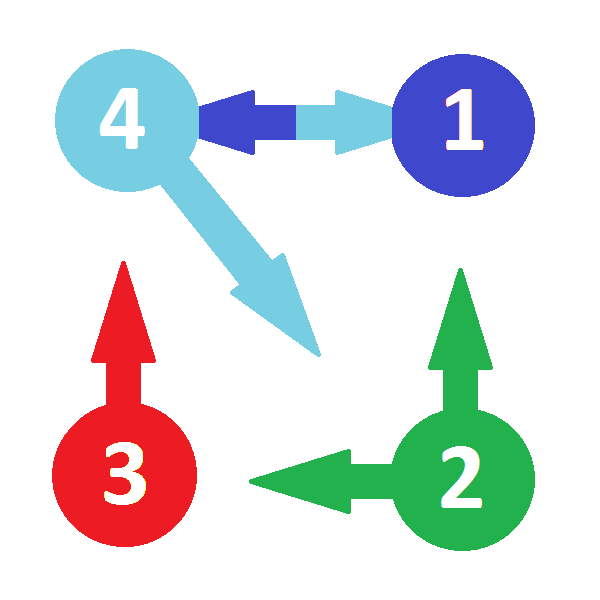
\includegraphics[scale=0.25]{figures/grafo}
	%\caption{Sergey Brin e Lawrence Page.}
	%{\scriptsize Grafo representando \textit{links} entre p\'aginas da \textit{web}}
	\label{}
\end{figure}	

\vspace{-0.5cm}

\begin{equation}\label{x0}
x_0 = \begin{pmatrix}
0\\ 0\\ 0\\ 1
\end{pmatrix}.
\end{equation}
	
\end{frame}
%%%%%%%%%%%%%%%%%%%%%%%%%%%%%%%%%%%%%%%%%%%%%%%%%%%%%%%%%%%%%%%%%%%%%%%%%%%%%%%%%%%%%%%%%%%%%%%%%%%%%%%%%%%%
%%%%%%%%%%%%%%%%%%%%%%%%%%%%%%%%%%%%%%%%%%%%%%%%%%%%%%%%%%%%%%%%%%%%%%%%%%%%%%%%%%%%%%%%%%%%%%%%%%%%%%%%%%%%
\begin{frame}
	%\section{Simulações}
	%\subsection{Simulação do Power Method}
	\frametitle{Simulação do Power Method}
	
\begin{figure}[!htb]
	\centering
	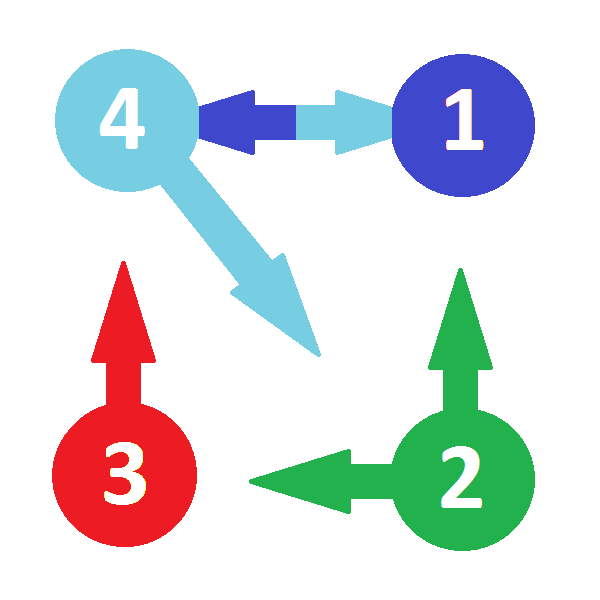
\includegraphics[scale=0.25]{figures/grafo}
	\hspace{0.1cm}
	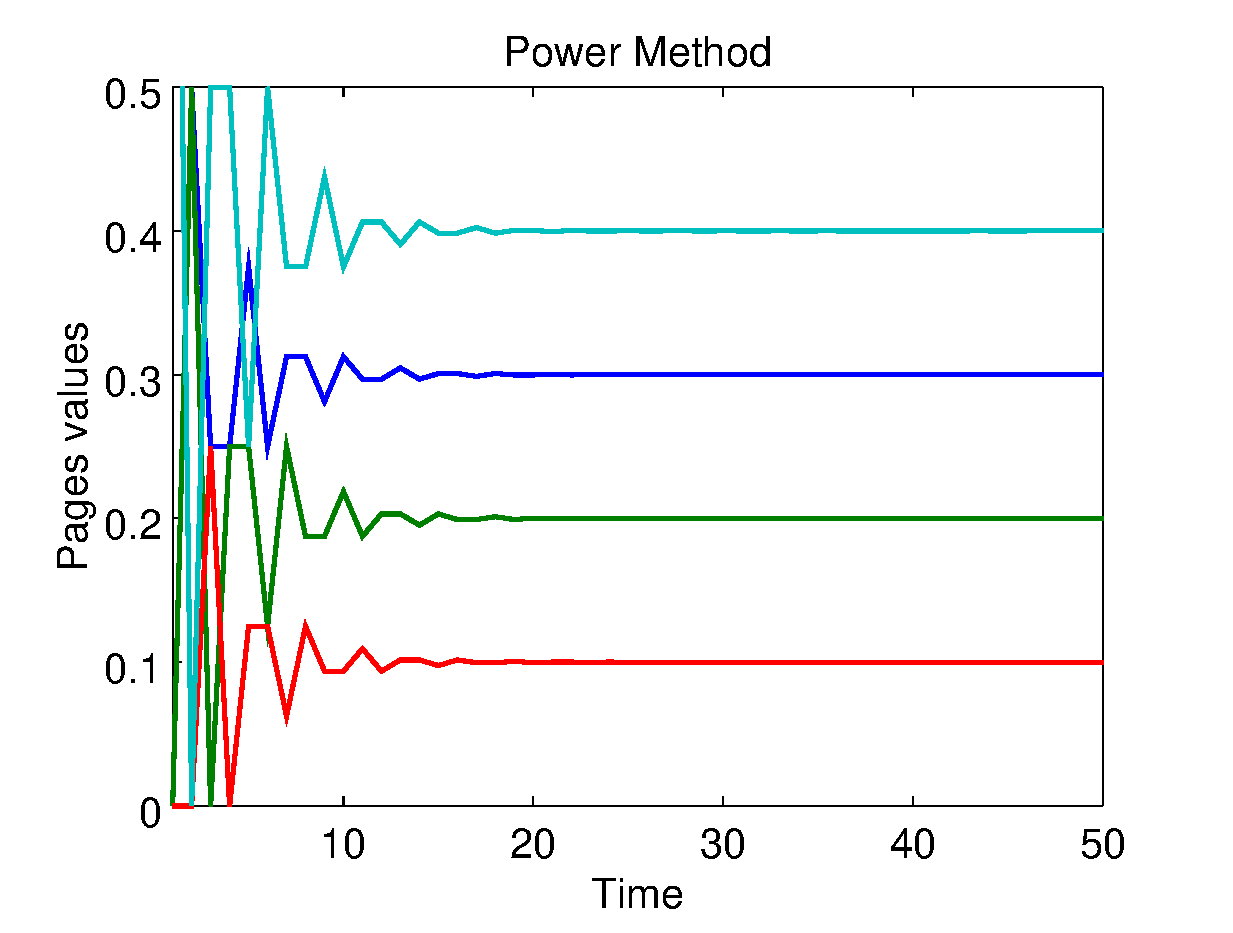
\includegraphics[scale=0.25]{figures/50/powermetod.eps}
	%\caption{Sergey Brin e Lawrence Page.}
	%{\scriptsize Grafo representando \textit{links} entre p\'aginas da \textit{web}}
	\label{}
\end{figure}	
	
\end{frame}
%%%%%%%%%%%%%%%%%%%%%%%%%%%%%%%%%%%%%%%%%%%%%%%%%%%%%%%%%%%%%%%%%%%%%%%%%%%%%%%%%%%%%%%%%%%%%%%%%%%%%%%%%%%%
%%%%%%%%%%%%%%%%%%%%%%%%%%%%%%%%%%%%%%%%%%%%%%%%%%%%%%%%%%%%%%%%%%%%%%%%%%%%%%%%%%%%%%%%%%%%%%%%%%%%%%%%%%%%
\begin{frame}
	%\section{Simulações}
	%\subsection{Simulação do \textit{Teleportation Model}}
	\frametitle{Simulação do \textit{Teleportation Model}}
	
	\vspace{-0.5cm}
\begin{figure}[!htb]
	\centering
	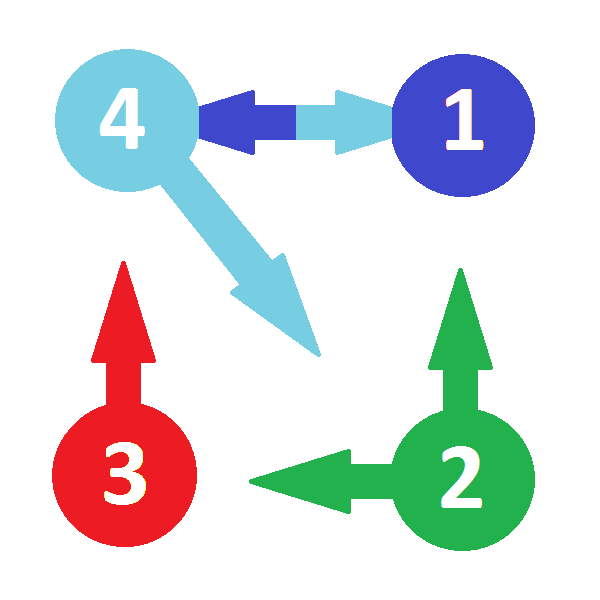
\includegraphics[scale=0.2]{figures/grafo}\\
	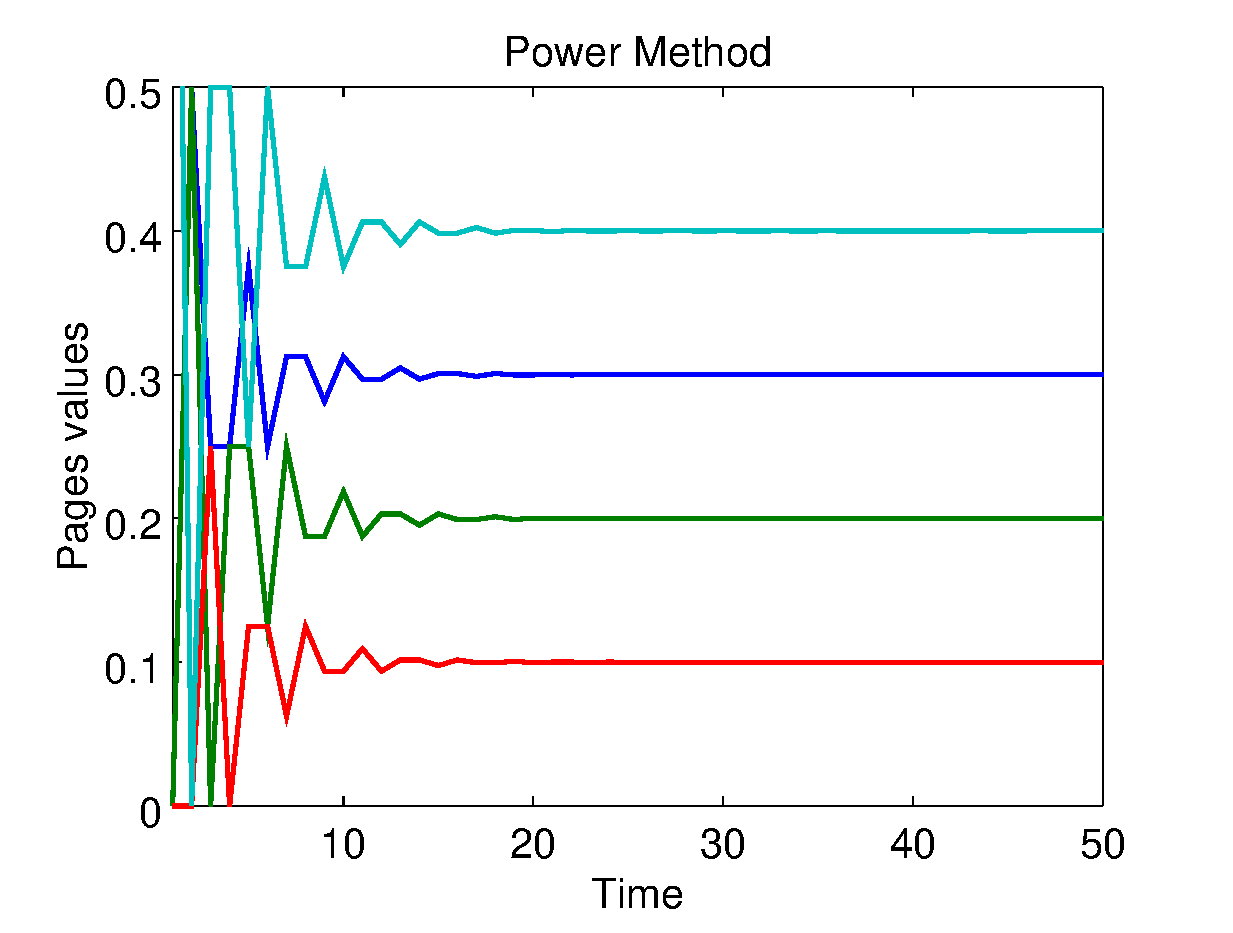
\includegraphics[scale=0.25]{figures/50/powermetod.eps}
	\hspace{0.1cm}
	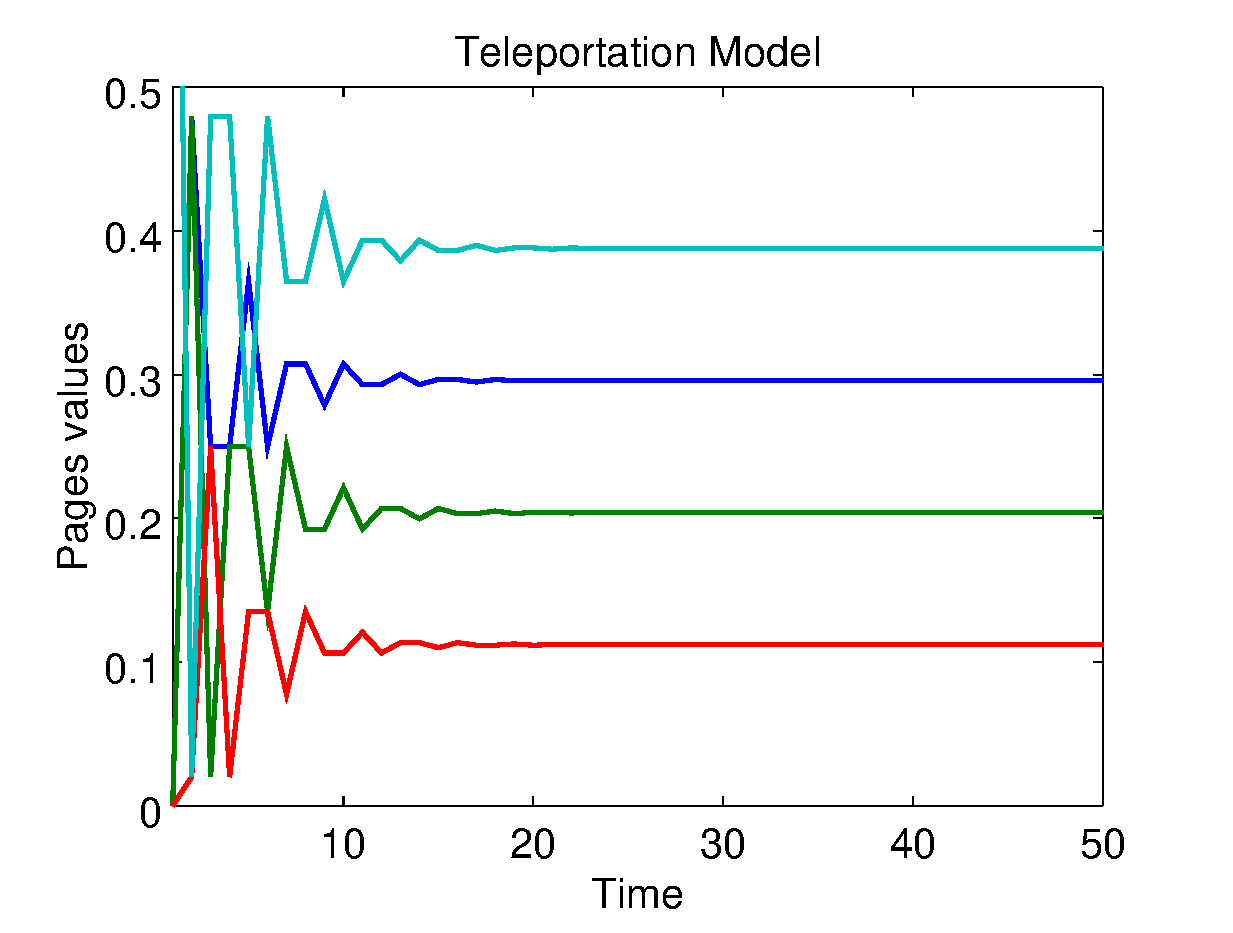
\includegraphics[scale=0.25]{figures/50/teleportation.eps}
	%\caption{Sergey Brin e Lawrence Page.}
	%{\scriptsize Grafo representando \textit{links} entre p\'aginas da \textit{web}}
	\label{}
\end{figure}	
	
\end{frame}
%%%%%%%%%%%%%%%%%%%%%%%%%%%%%%%%%%%%%%%%%%%%%%%%%%%%%%%%%%%%%%%%%%%%%%%%%%%%%%%%%%%%%%%%%%%%%%%%%%%%%%%%%%%%
%%%%%%%%%%%%%%%%%%%%%%%%%%%%%%%%%%%%%%%%%%%%%%%%%%%%%%%%%%%%%%%%%%%%%%%%%%%%%%%%%%%%%%%%%%%%%%%%%%%%%%%%%%%%
\begin{frame}
	%\section{Simulações}
	%\subsection{Simulação do Modelo Distribuído}
	\frametitle{Simulação do Teleportation Model Distribuído}

\begin{figure}[!htb]
	\centering
	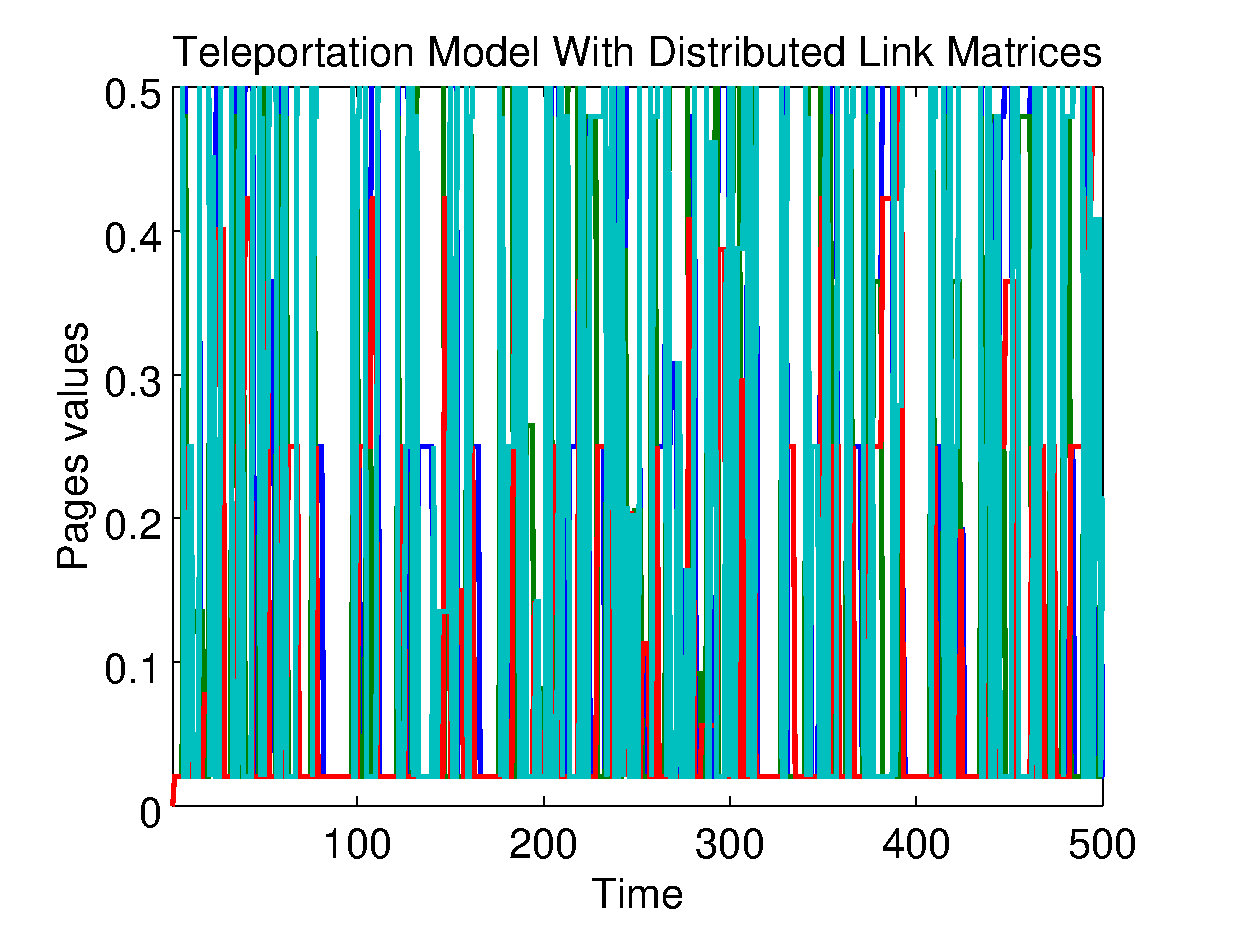
\includegraphics[scale=0.4]{figures/500/teledistributed}
	%\caption{Sergey Brin e Lawrence Page.}
	%{\scriptsize Grafo representando \textit{links} entre p\'aginas da \textit{web}}
	\label{}
\end{figure}	
	
\end{frame}
%%%%%%%%%%%%%%%%%%%%%%%%%%%%%%%%%%%%%%%%%%%%%%%%%%%%%%%%%%%%%%%%%%%%%%%%%%%%%%%%%%%%%%%%%%%%%%%%%%%%%%%%%%%%
%%%%%%%%%%%%%%%%%%%%%%%%%%%%%%%%%%%%%%%%%%%%%%%%%%%%%%%%%%%%%%%%%%%%%%%%%%%%%%%%%%%%%%%%%%%%%%%%%%%%%%%%%%%%
\begin{frame}
	%\section{Simulações}
	%\subsection{Simulação do Modelo Distribuído}
	\frametitle{Simulação do Teleportation Model Distribuído}

\begin{itemize}
	\item A falta de convergência é tipica de simulações estocásticas.
\end{itemize}

\begin{figure}[!htb]
	\centering
	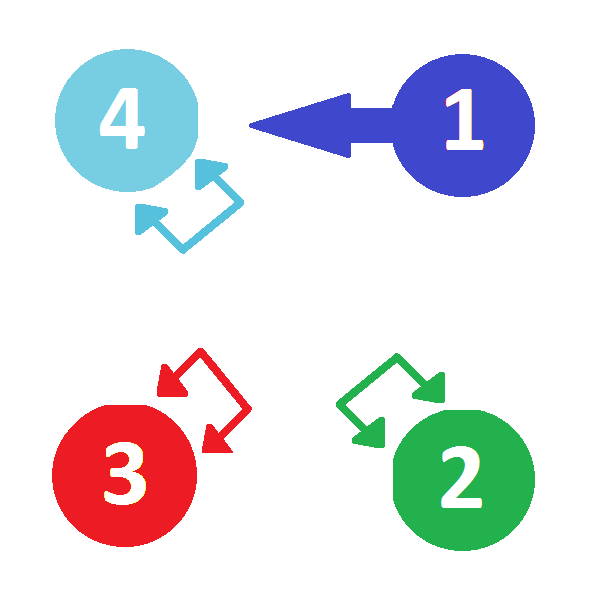
\includegraphics[scale=0.20]{figures/loop}
	%\caption{Sergey Brin e Lawrence Page.}
	%{\scriptsize Grafo representando \textit{links} entre p\'aginas da \textit{web}}
	\label{}
\end{figure}

\vspace{-0.5cm}

\begin{equation}\nonumber
A_1 = \begin{pmatrix}
 0 & 0 & 0 &  0 \\
 0 & 1 & 0 &  0 \\
 0 & 0 & 1 &  0  \\
 1 & 0 & 0 &  1
\end{pmatrix}
\end{equation}		
	
\end{frame}
%%%%%%%%%%%%%%%%%%%%%%%%%%%%%%%%%%%%%%%%%%%%%%%%%%%%%%%%%%%%%%%%%%%%%%%%%%%%%%%%%%%%%%%%%%%%%%%%%%%%%%%%%%%%
%%%%%%%%%%%%%%%%%%%%%%%%%%%%%%%%%%%%%%%%%%%%%%%%%%%%%%%%%%%%%%%%%%%%%%%%%%%%%%%%%%%%%%%%%%%%%%%%%%%%%%%%%%%%
\begin{frame}
	%\section{Simulações}
	%\subsection{Simulação do Modelo Distribuído}
	\frametitle{O Modelo Recursivo da Média no Tempo Aplicada a Simulação do Modelo Distribuído}
	
	\vspace{-0.5cm}
\begin{figure}[!htb]
	\centering
	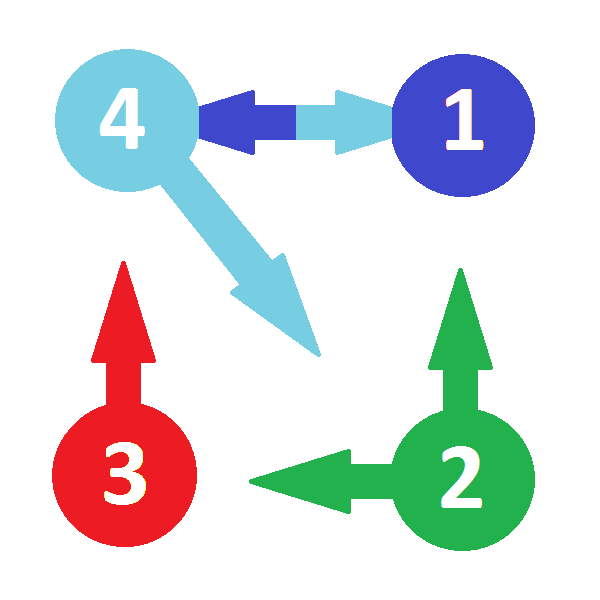
\includegraphics[scale=0.2]{figures/grafo}\\
	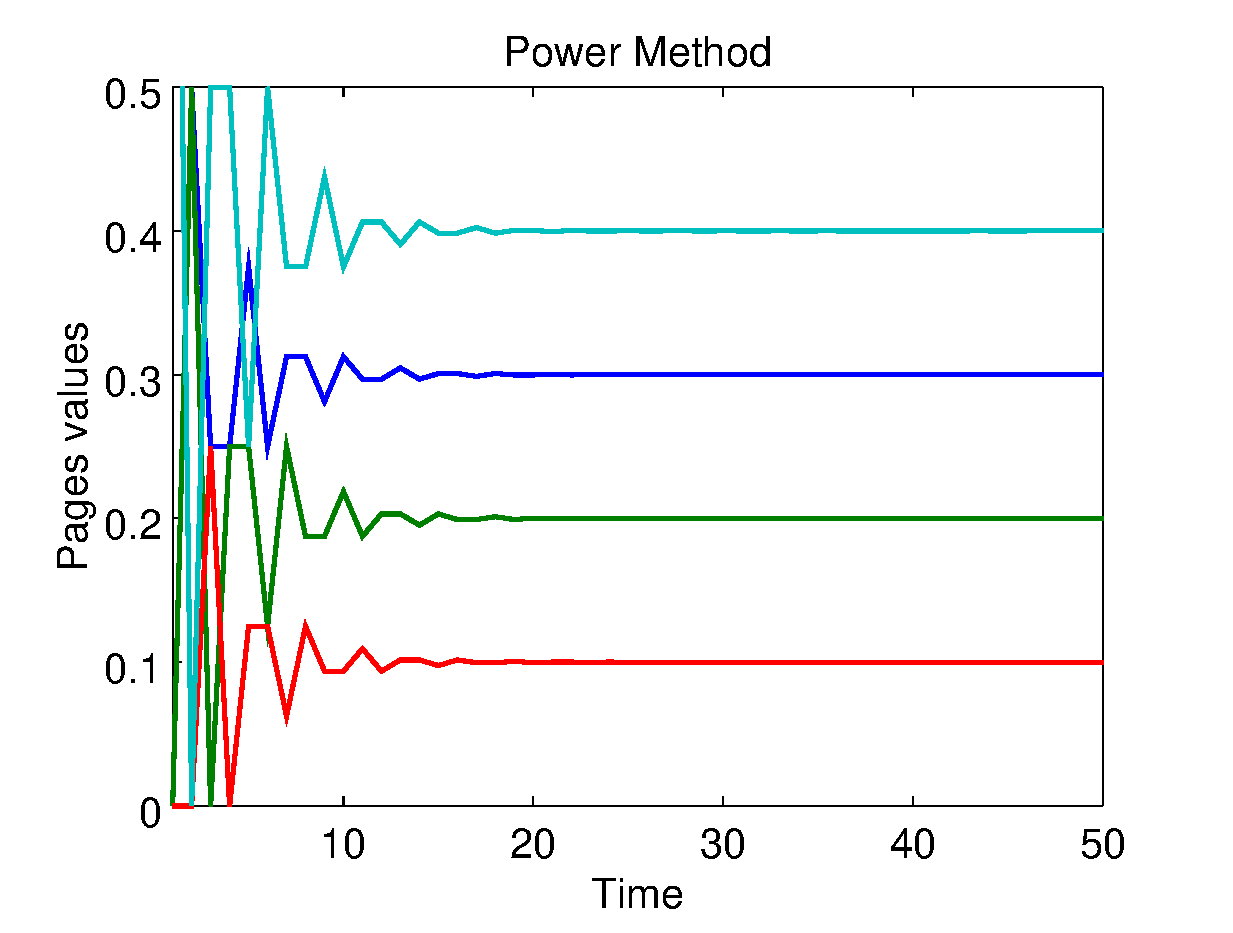
\includegraphics[scale=0.25]{figures/50/powermetod.eps}
	\hspace{0.1cm}
	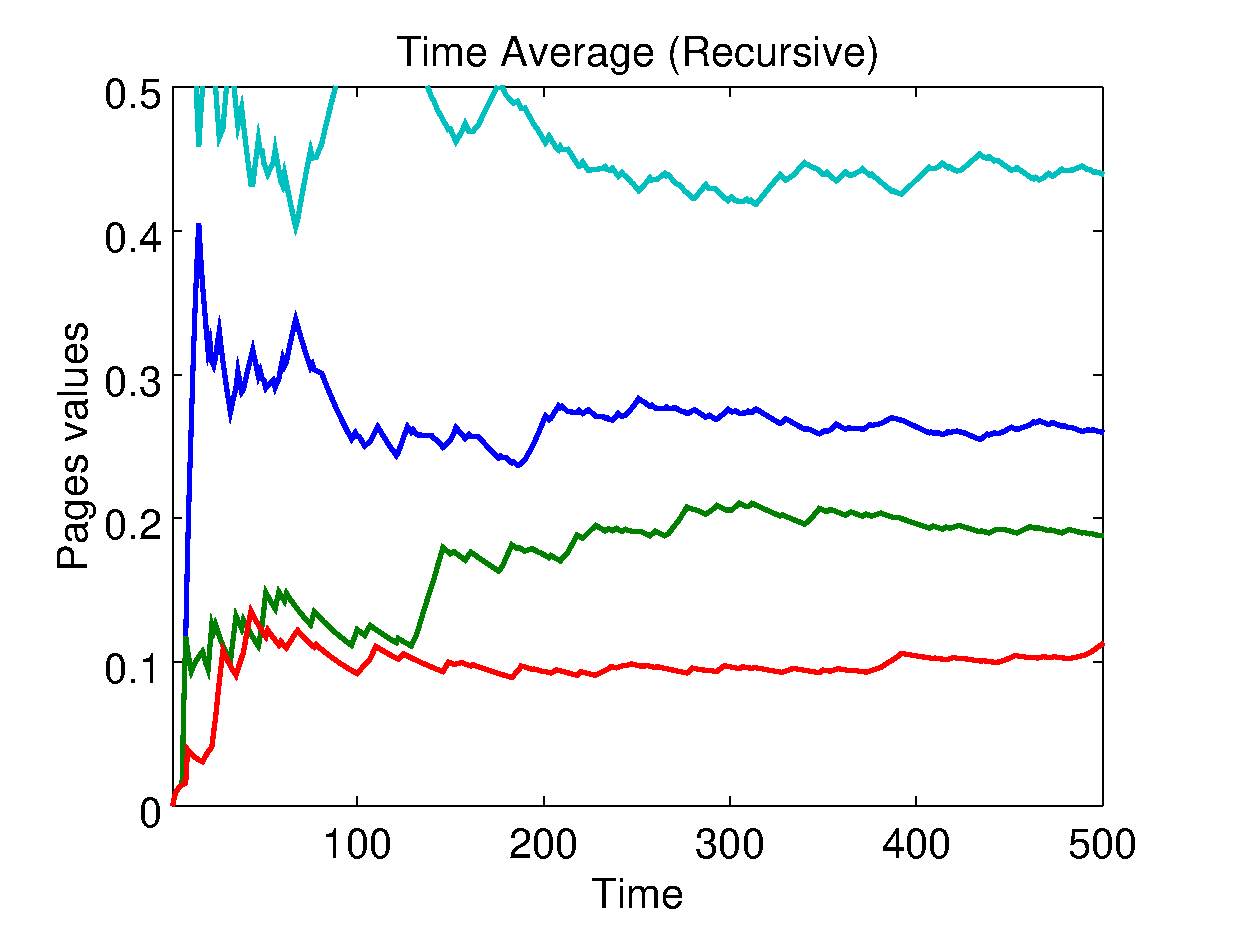
\includegraphics[scale=0.25]{figures/500/timerecursive.eps}
	%\caption{Sergey Brin e Lawrence Page.}
	%{\scriptsize Grafo representando \textit{links} entre p\'aginas da \textit{web}}
	\label{}
\end{figure}	
	
\end{frame}
%%%%%%%%%%%%%%%%%%%%%%%%%%%%%%%%%%%%%%%%%%%%%%%%%%%%%%%%%%%%%%%%%%%%%%%%%%%%%%%%%%%%%%%%%%%%%%%%%%%%%%%%%%%%
%%%%%%%%%%%%%%%%%%%%%%%%%%%%%%%%%%%%%%%%%%%%%%%%%%%%%%%%%%%%%%%%%%%%%%%%%%%%%%%%%%%%%%%%%%%%%%%%%%%%%%%%%%%%
\begin{frame}
	%\section{Simulações}
	%\subsection{Método de Monte Carlo Aplicado após Modelo Recursivo da Média}
	\frametitle{Método de Monte Carlo Aplicado após Modelo Recursivo da Média}
	
	\vspace{-0.5cm}
\begin{figure}[!htb]
	\centering
	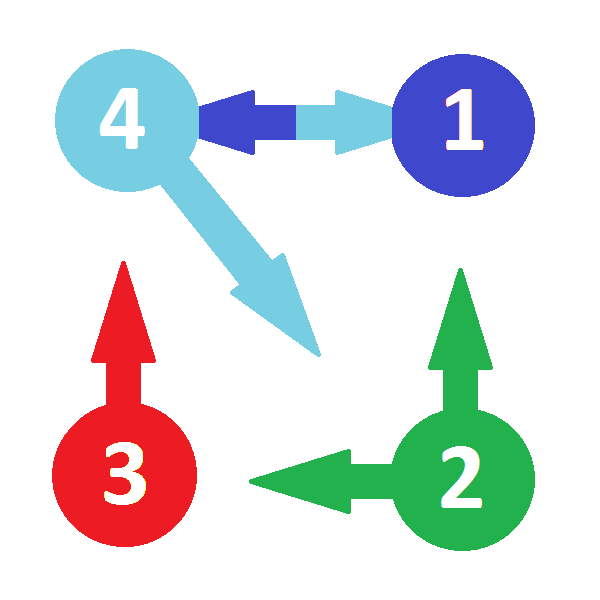
\includegraphics[scale=0.2]{figures/grafo}
	\hspace{1cm}
	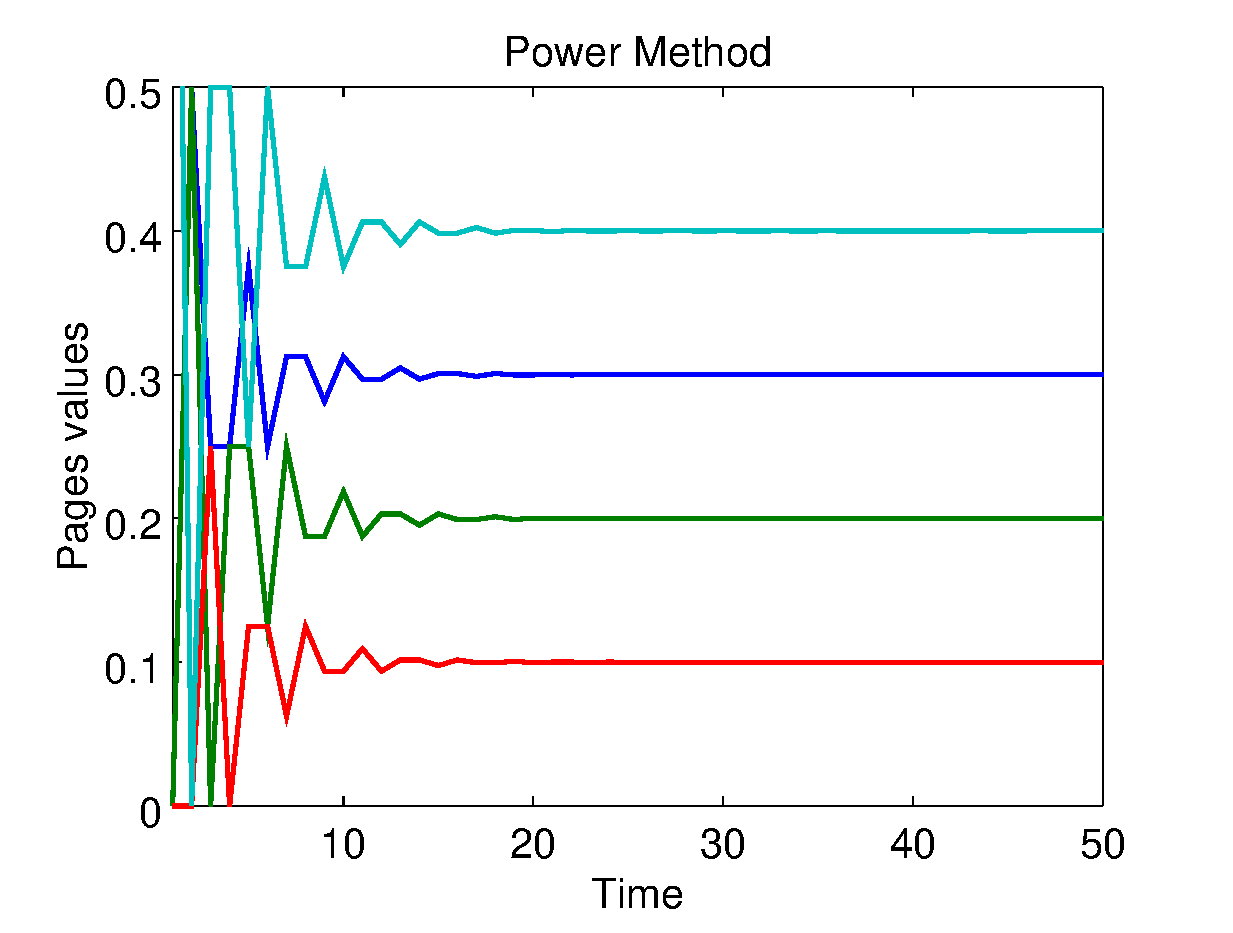
\includegraphics[scale=0.2]{figures/50/powermetod.eps}\\
	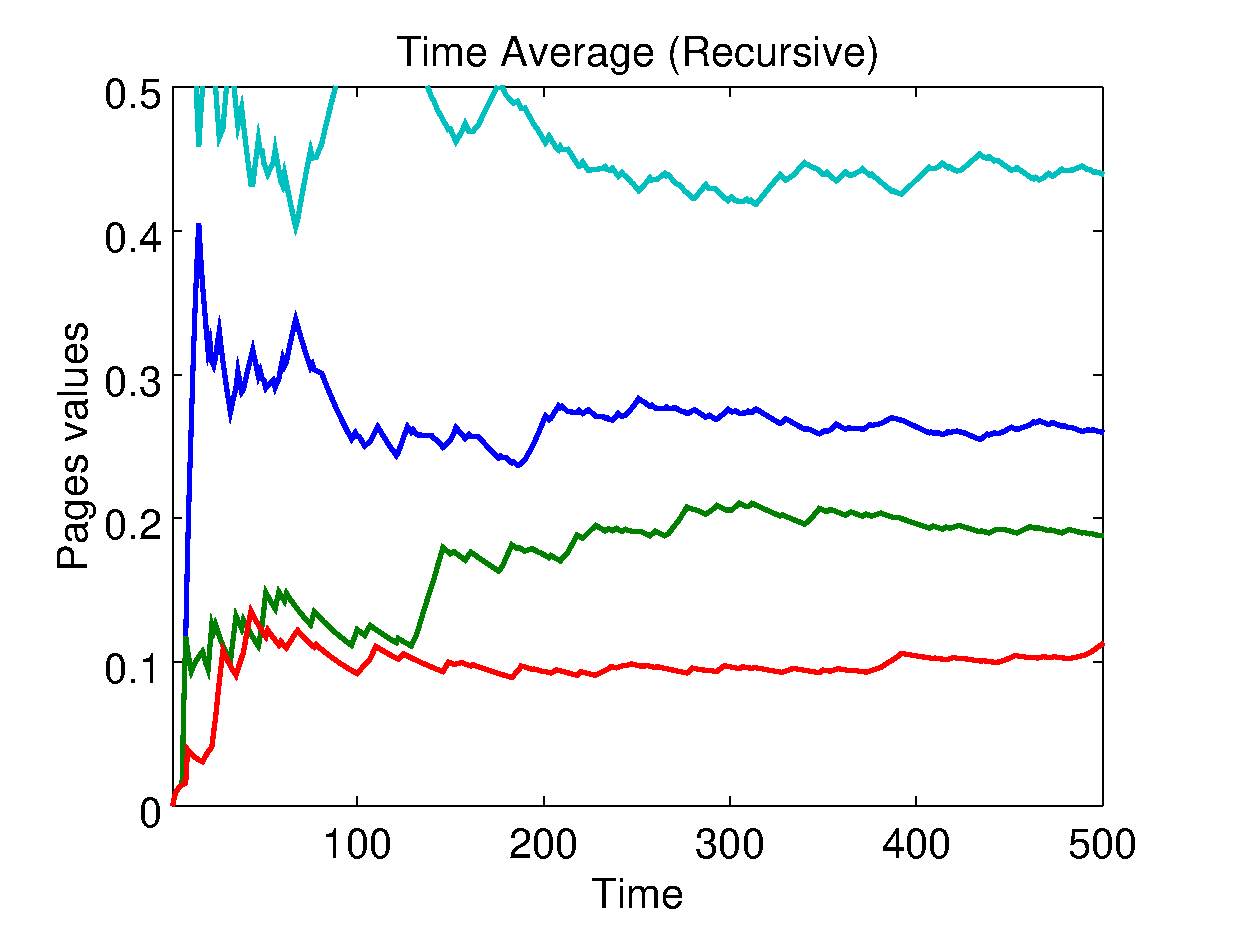
\includegraphics[scale=0.2]{figures/500/timerecursive.eps}
	\hspace{0.1cm}
	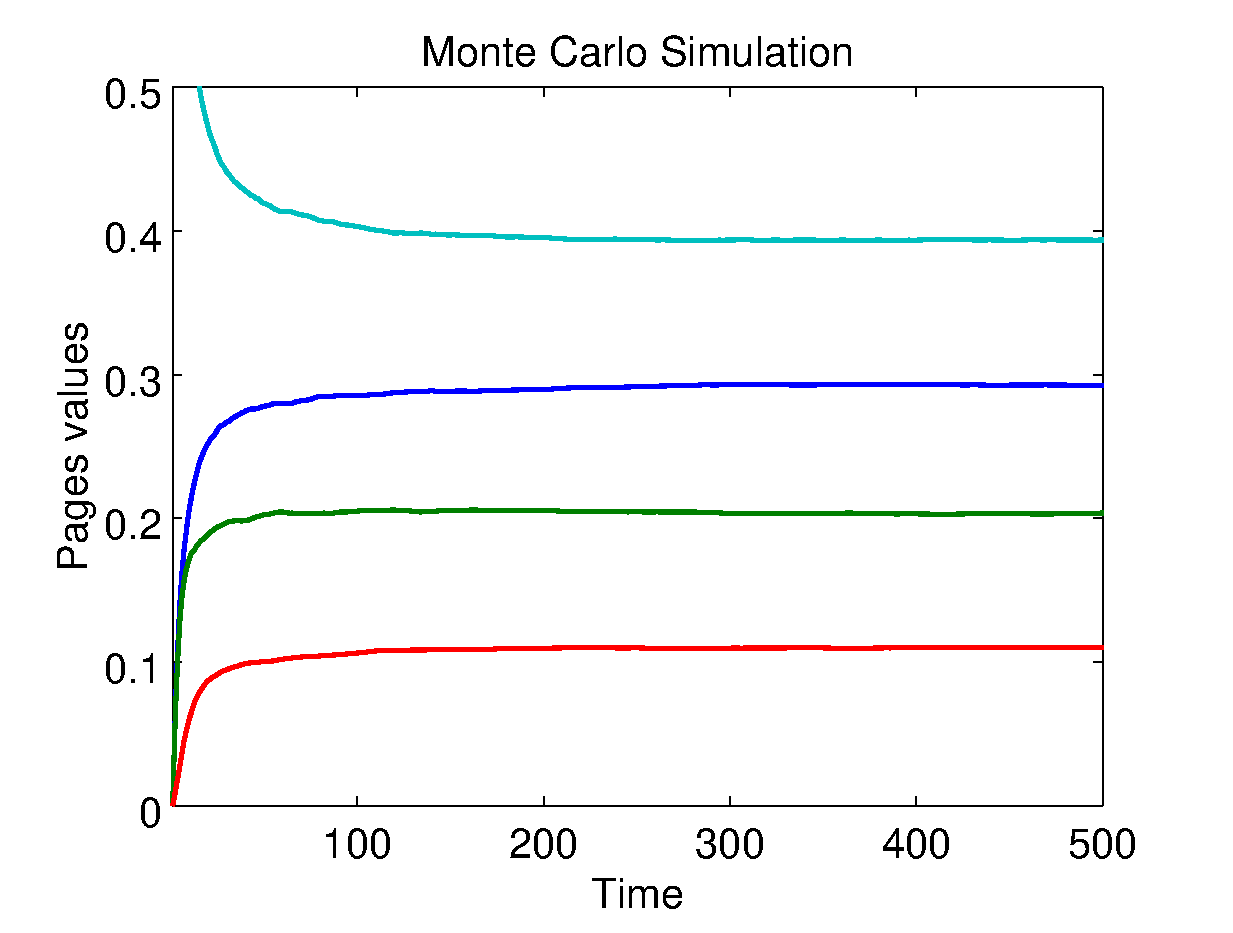
\includegraphics[scale=0.2]{figures/500/montecarlo.eps}
	%\caption{Sergey Brin e Lawrence Page.}
	%{\scriptsize Grafo representando \textit{links} entre p\'aginas da \textit{web}}
	\label{}
\end{figure}	
	
\end{frame}
%%%%%%%%%%%%%%%%%%%%%%%%%%%%%%%%%%%%%%%%%%%%%%%%%%%%%%%%%%%%%%%%%%%%%%%%%%%%%%%%%%%%%%%%%%%%%%%%%%%%%%%%%%%%
%%%%%%%%%%%%%%%%%%%%%%%%%%%%%%%%%%%%%%%%%%%%%%%%%%%%%%%%%%%%%%%%%%%%%%%%%%%%%%%%%%%%%%%%%%%%%%%%%%%%%%%%%%%%
\begin{frame}
	\section{Considerações Finais}
	\frametitle{Considerações Finais}

\begin{itemize}
	\item O sucesso dos sistemas de busca.
	
	\vspace{0.5cm}	

	\item Utilizar outros m\'etodos, válidos na simulação do \textit{PageRank}.
		
	\vspace{0.5cm}

	\item Implementação com \textit{links} já coletados por um \textit{Web Crawling}\footnote{\tiny \justifying U.K. New Zealand Univ., Statistical Cybermetrics Research Group, 2006.}.
	
	\begin{itemize}
		\item Uso de outras linguagens de programação.
		\item Computação Distribuída.
	\end{itemize}
\end{itemize}		
	
\end{frame}
%%%%%%%%%%%%%%%%%%%%%%%%%%%%%%%%%%%%%%%%%%%%%%%%%%%%%%%%%%%%%%%%%%%%%%%%%%%%%%%%%%%%%%%%%%%%%%%%%%%%%%%%%%%%
%%%%%%%%%%%%%%%%%%%%%%%%%%%%%%%%%%%%%%%%%%%%%%%%%%%%%%%%%%%%%%%%%%%%%%%%%%%%%%%%%%%%%%%%%%%%%%%%%%%%%%%%%%%%

\end{document}